% 90-09(90쪽) — 반지름의 길이가 4 인 원에 내접하는 삼각형 ABC(중심에서 C 로 가는 점선 반지름). 스캔 화질이 낮아 TikZ 로 다시 그림.
% 라벨은 원문 그대로 A·B·C 와 4(반지름)·60°(∠A)·45°(∠B) 만. AB 의 길이는 적지 않는다.
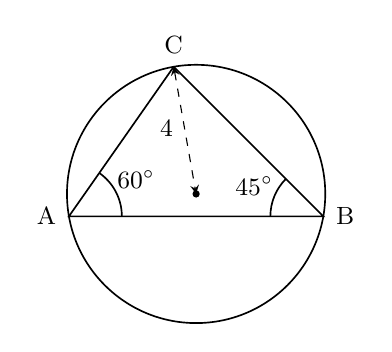
\begin{tikzpicture}[scale=0.82, line width=0.6pt]
  \draw (0,0) circle (2.0);
  \coordinate (C) at (-0.347,1.970);
  \coordinate (A) at (-1.970,-0.347);
  \coordinate (B) at (1.970,-0.347);
  \draw (C) -- (A) -- (B) -- (C);
  \fill (0,0) circle (1.6pt);
  \draw[dashed, line width=0.4pt, <->, >=stealth] (C) -- (0,0);
  \draw (A) ++(0:0.82) arc (0:55:0.82);
  \draw (B) ++(180:0.82) arc (180:135:0.82);
  \node[above=1pt, font=\small] at (C) {$\mathrm{C}$};
  \node[left=1pt, font=\small] at (A) {$\mathrm{A}$};
  \node[right=1pt, font=\small] at (B) {$\mathrm{B}$};
  \node[font=\small] at (-0.46,1.02) {$4$};
  \node[font=\small] at (-0.93,0.22) {$60^\circ$};
  \node[font=\small] at (0.90,0.12) {$45^\circ$};
\end{tikzpicture}
